\documentclass[12pt]{article}
\usepackage[latin1]{inputenc}

\usepackage[dvips]{graphics,graphicx,epsfig}
%\usepackage{amssymb}
\usepackage{amsmath}
%\usepackage{graphics}

%%%%%%%%%%%%%%%%%%%%%%%%%%%%%%%%%%%%%%%%%%%%%%%%%%%%%%%%%%%%%%%%%
\usepackage{amssymb, amsmath, latexsym, amsbsy,amsthm}
\usepackage{amsfonts}
\usepackage[T1]{fontenc}
\usepackage{amscd}
\usepackage{graphicx}
\usepackage{latexsym}
\usepackage{siunitx}
\usepackage{color}
\usepackage{here}
\usepackage{color}
\usepackage{tikz}
\usepackage[colorlinks]{hyperref}
\usepackage{subeqnarray}
\usepackage{eqnarray}
\usepackage{pxfonts}
\usepackage{epsfig}
\usepackage{lineno}
\newcommand{\N}{\mathbb{N}}
\usepackage{color}
\usepackage[colorlinks]{hyperref}
\hypersetup{colorlinks=true,linkcolor=red}
\textheight=23.5cm \textwidth=17cm \frenchspacing
\linespread{1.05}
%
\newcommand{\U}{\mathcal{U}}
\newcommand{\Z}{\mathbb{Z}}
\newcommand{\Q}{\mathbb{Q}}
\newcommand{\R}{\mathbb{R}}
\newcommand{\C}{\mathbb{C}}
%
\textheight240mm \voffset-23mm \textwidth160mm \hoffset-20mm
\oddsidemargin20mm \evensidemargin20mm \baselineskip10cm
%
\newtheorem{dfn}{Definition}
\newtheorem{theorem}{Theorem}
\newtheorem{lem}{Lemma}
\newtheorem{cor}{Corollary}
\newtheorem{rem}{Remark}
\newtheorem{prop}{Proposition}
\newtheorem{prv}{Proof}
%
\newcommand{\bpf}{{\sl Proof :}\hspace{5mm}}
\setlength{\unitlength}{1mm} \columnsep6mm
%\documentclass[a4paper, 11pt]{article}
%\usepackage[english]{babel}
%\usepackage[T1]{fontenc}
%\usepackage[latin1]{inputenc}
%\usepackage{fullpage}
%\usepackage{tikz}
%\usepackage{lmodern} 
%\usepackage{graphicx} 
%\usepackage{amsmath}
%\usepackage{amsthm}
%\usepackage{natbib}
%\usepackage{amsfonts}
%\usepackage{subfigure}
%\usepackage{epsfig}
%\usepackage{here}
%\usepackage{float}
%%\usepackage[backend=biber]{biblatex}
%\newtheorem{de}{Definition}[section]
%\newtheorem{theo}{Theorem}[section]    
%\newtheorem{lem} {Lemma}[section]  
%\newtheorem{pro}{Proposition}[section]
%\newtheorem{co}{corollary}[section]
%\setcounter{tocdepth}{3}
%
%\textheight240mm \voffset-23mm \textwidth160mm \hoffset-20mm
%\oddsidemargin20mm \evensidemargin20mm \baselineskip10cm

\author{\bf  Fidelette Chezeu Toumeni$^{1,2}$, Samuel Bowong$^{1,2,3}$Andr\'{e} Nana Yakam$^{1,2,\dag}$ \\
{\small $^1$ Laboratory of   Mathematics,
Department of Mathematics and Computer Science,}\\
{\small $^2$ University of Douala, PO Box 24157  Douala, Cameroon}\\
%{\small $^2$ }\\
\small{$^3$ UMI 209 IRD \& UPMC UMMISCO, Bondy, France}\\
\small{Project team GRIMCAPE-Cameroon}\\
{\small $^\dag$ Corresponding author: Tel. +237 677 86 95 39 }\\
{\small Email: sbowong@gmail.com}}
\date{}
\title{ \textbf{Parameter estimation of a tuberculosis model in a patchy
environment: case of Cameroon}}
\begin{document}
\baselineskip 6mm
\maketitle

\date{}
%\tableofcontents 
 
%\pagestyle{plain}
\begin{abstract}
\noindent

\end{abstract}

\section{Introduction}

\section{ Model formulation }
\noindent

In this section, we proceed to the formulation of a mathematical patch model of the spread of tuberculosis disease in Cameroon. The model is based on the interaction between the populations of the different cities of the country. To do so, we use the compartmental modelling approach with a meta population. We consider the following compartments.

\subsection{Meta population model}
\noindent 

Our model is strongly based on the patches model formulates and studied by D.P. Moualeu and al (2013)\cite{1} , and notations and indices are all preserved. therefore, D.P. Moualeu and al\cite{1} in his study, had not taken into account the reinfection that accurs during the contact between a latent and an infectious person. Thus, taking into account this reinfection is the reason of being of our current study.

Consider a population divided into several subgroups called patches, which the total human population present in each patch $i$ at time $t$ is denoted by $N_{i}$, for $i = 1,...,n$: we use an n-patches of TB disease dynamics. 
 
In this model, we do not take into account the place of residence of an individual.
But, we just considers where he is at time t. The transfer rate from a
patch $i$ to a patch $j$, for $i \neq j$, is denoted by $m_{ji} \geqslant 0$. We assume that infection and death due to disease do not occur during the move. 
 Thus, the dynamics of the total population in the patch $i$ at time $t$ is given by:
 \begin{equation}
\dot{N}_{i}= \Psi_{i}-\mu_{i}N_{i}+\sum_{j=1;j\neq i}^{n}m_{ij}N_{j}-N_{i}\sum_{j=1; j\neq i}^{n}m_{ji}\,\,\,\,for\,\,\,\ i = (1,\cdots,n),
\label{1}
 \end{equation}
 
where $\mu_{i}$ denotes the natural mortality rate of individuals in patch $i$, and $\psi_{i}$ the recruitment rate inside the population of patch $i$.

Then, the model system  (\ref{1}) can be written in the following compact form:

\begin{equation}
\label{e4}
\dot{N}=\psi - diag(\mu)N + \mathcal{M}N,
\end{equation}

where, $N= ( N_{1},N_{1},\cdots,N_{n})^{T}$, $\psi= ( \psi_{1},\cdots, \psi_{n})^{T}$, $\mu=( \mu_{1}, \cdots, \mu_{n})^{T}$. The matrix $\mathcal{M}$ is defined by: $\mathcal{M}_{i,j}=m_{ij}$ for $i\neq j$, and $\mathcal{M}(i,i)=-\sum_{j=1;j\neq i}^{n}m_{ji}$. $diag(\mu)$ defined  the diagonal matrix with $\mu_{i}$ as its $(i; i)$ entry.


\subsection{Multigroup model}
In the epidemiological literature, the term "multigroup" usually refers to the division of a heterogeneous population into several homogeneous groups based on individual behaviour. Each group is then subdivided into epidemiological compartments\cite{1}.

The population of each patch is subdivided into several classes: 
\begin{enumerate}
\item The class of susceptible ($S$)\\
This class is made up of people who are healthy but at risk of contracting the disease. We denote by $S(t)$, the number of persons at risk at time t and $S_{i}$ the susceptible in the patch $i$.
\item The class of latently infected  ($E$)\\
This class is composed by persons exposed to TB, but not infectious.
Then, $E(t)$ represent the number of  latently infected at time $t$ and $E_{i}$ the latently in the patch $i$.
\item The class of diagnosed infectious ($I$)\\
It's the class of persons who have an active TB confirmed
after a sputum examination at the hospital. $I(t)$ is therefore the number of diagnosed infectious at time $t$ and $I_{i}$ the diagnosed infectious in the patch $i$.
\item The class of undiagnosed infectious ($J$)\\
It's the class of persons who have
an active TB not confirmed by a sputum examination at the hospital.
$J(t)$ is the number of undiagnosed infectious at time $t$ and $J_{i}$ the  undiagnosed in the patch $i$.
\item The class of recovered individuals ($R$)\\
This class is composed by the persons cured after a therapy of treatment in the hospital. $R(t)$ represent the number of persons who have recovered individuals at time $t$ and $R_{i}$, the recovered individuals in the patch $i$.
\end{enumerate}

Thus, the total population in the $i$ at time $t$ is defined by:
\begin{equation}
N_{i}(t)= S_{i}(t)+E_{i}(t)+I_{i}(t)+J_{i}(t)+R_{i}(t)
\end{equation}

In addition to these classes the following assumptions have been made:
\begin{itemize}
\item Since diagnosed infectious have been detected in the health centers, we assume that the transmission of the infection from diagnosed infectious to susceptible individuals is assumed to be frequency-dependent (limited). Indeed, diagnosed infectious are educated from TB disease so that they can avoid contacts with susceptible individuals. 
\item While the TB transmission from undiagnosed infectious to susceptible individuals is assumed to be density-dependent ( non-limited). Since some undiagnosed infectious do not know their
TB-status, people around them are not aware of their TB-status, and thus interact with them naturally.

\end{itemize}

Figure \ref{fig1}  presents the compartmental diagram of the model.
\begin{figure}[h!]
\begin{center}
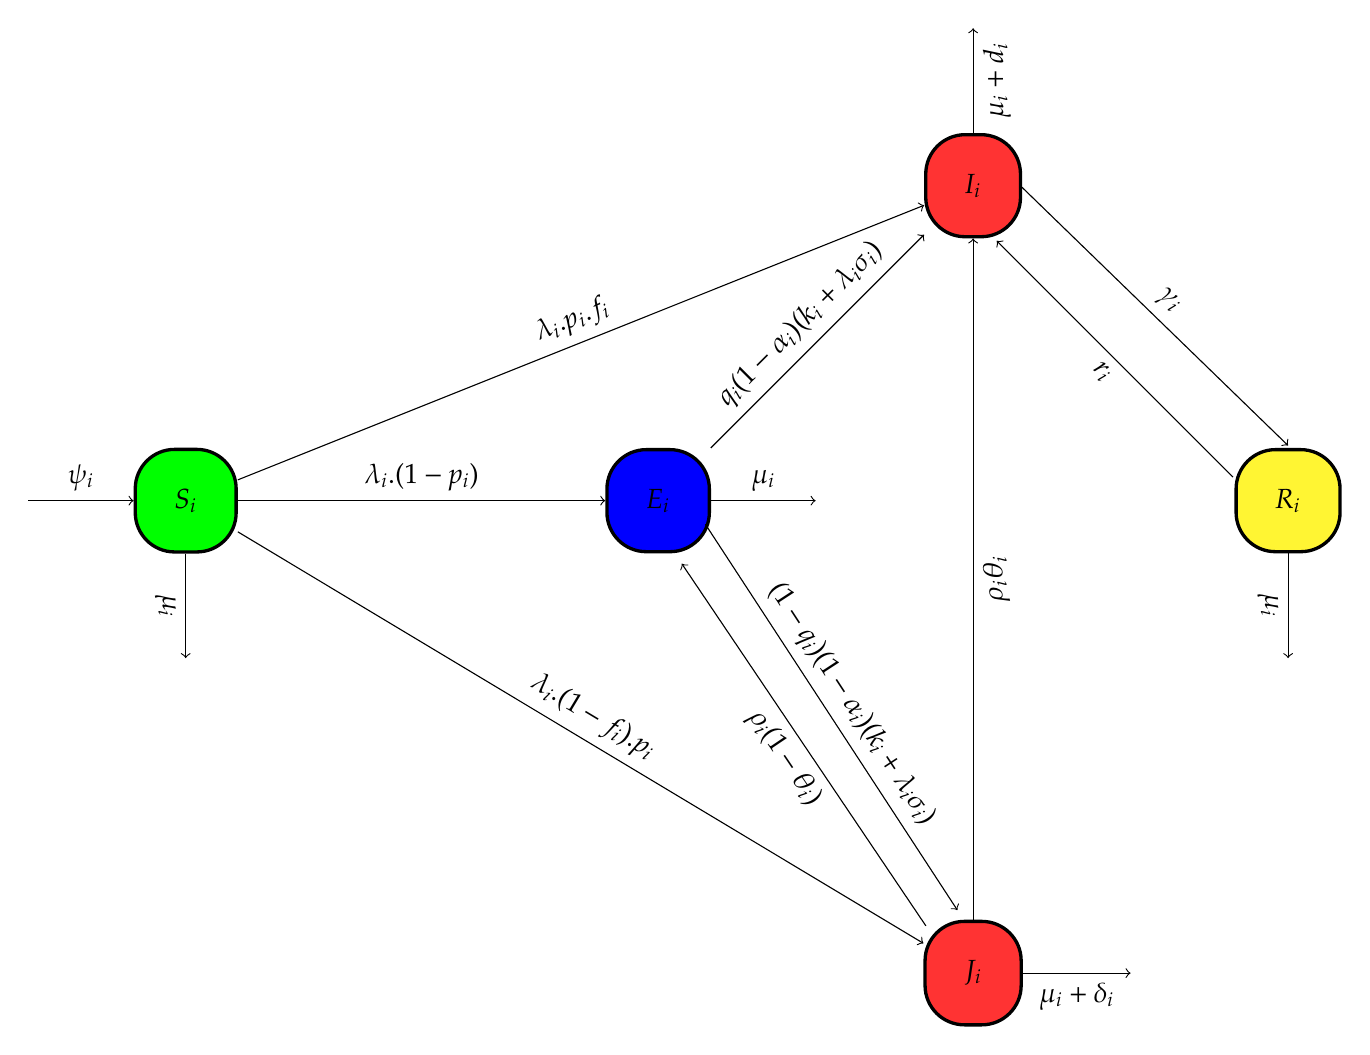
\begin{tikzpicture}
\node[very thick, black, rectangle,fill=green,inner sep=0.5cm,rounded corners=0.5cm, draw] (b) at (3,0) {$S_{i}$};
\node[very thick, black, rectangle,fill=blue,inner sep=0.5cm,rounded corners=0.5cm, draw] (c) at (9,0) {$E_{i}$};
\node[very thick, black, rectangle,fill=yellow!80,inner sep=0.5cm,rounded corners=0.5cm, draw] (e) at (17,0) {$R_{i}$};
\node[very thick, black, rectangle,fill=red!80,inner sep=0.5cm,rounded corners=0.5cm, draw] (f) at (13,4) {$I_{i}$};
\node[very thick, black, rectangle,fill=red!80,inner sep=0.5cm,rounded corners=0.5cm, draw] (g) at (13,-6) {$J_{i}$};
\draw[->] (b)--node[midway, above, sloped]{$\lambda_{i}.p_{i}.f_{i}$} (f);
%\draw[->, dashed] (d)--(c);
\draw[->] (b)--node[midway, above, sloped]{$\lambda_{i}.(1-f_{i}).p_{i}$} (g);
\draw[->] (b)--node[midway, above, sloped]{$\lambda_{i}.(1-p_{i})$} (c);
\draw[->] (c)--node[midway, above, sloped]{$q_{i}(1-\alpha_{i})(k_{i}+ \lambda_{i}\sigma_{i}) $}(f);

\draw[->] (9.6,-0.3)--node[midway, above, sloped]{$(1-q_{i})(1-\alpha_{i})(k_{i}+\lambda_{i}\sigma_{i})$}(12.8,-5.2);

\draw[<-] (9.3,-0.80)--node[midway, below, sloped]{$\rho_{i}(1-\theta_{i})$}(12.4,-5.4);

\draw[->] (13.6,4)--node[midway, above, sloped]{$\gamma_{i}$}(17,0.7);

\draw[<-] (13.3,3.3)--node[midway, below, sloped]{$r_{i}$}(16.3,0.3);

\draw[->] (g)--node[midway, below, sloped]{$\rho_{i}\theta_{i}$}(f);
%\draw[dashed] (11,0.7)--(11,1.5);
\draw[->] (1,0)--node[midway, above, sloped]{$\psi_{i}$}(b);
\draw[->] (c)--node[midway, above, sloped]{$\mu_{i}$}(11,0);
\draw[->] (b)--node[midway, below, sloped]{$\mu_{i}$}(3,-2);
\draw[->] (g)--node[midway, below, sloped]{$\mu_{i}+\delta_{i}$}(15,-6);
\draw[->] (f)--node[midway, below, sloped]{$\mu_{i}+d_{i}$}(13,6);
\draw[->] (e)--node[midway, below, sloped]{$\mu_{i}$}(17,-2);
%\draw[->] (13,0.3)-- (13,-0.3)node[right]{$\mu_{F_2}$};
\end{tikzpicture}
\end{center}
\caption{Structure of the model}
\label{fig1}
\end{figure}

Recruitment in each patch is into the susceptible classes and is at the constant rate $\psi_{i}$. The
constant rate for non-disease related death is $\mu_{i}$. Diagnosed and undiagnosed infectious have addition death rates due to disease with rates $ d_{i}$ and $\delta_{i}$, respectively. Transmission of TB bacteria occurs after adequate contacts between susceptible individuals, diagnosed and undiagnosed infectious. Then,
susceptible individuals of patch $i$ acquire TB infection from individuals with active TB at rate $\lambda_{i}$, given by:
\begin{equation}
\lambda_{i}=\beta_{i}^{I}\frac{I_{i}}{N_{i}}+ \beta_{i}^{J}J_{i},
\end{equation}
where, $\beta_{i}^{I}$ and $\beta_{i}^{J}$ are effective contact rates of diagnosed and undiagnosed
infectious that are sufficient to transmit the infection to a susceptible individual in patch $i$. $P_{i} $ is the Proportions of new infected among susceptible individuals assumed to undergo a fast progression of the disease and will transfer directly to the classes of infectious $I_{i}$ and $J_{i}$, while the remainder $(1-P_{i} )$ develops a latent TB and enter the latent class $E_{i}$.
 Latently infected individuals are assumed
to acquire some immunity as a result of the infection, which reduces the risk
of subsequent infection but does not fully prevent it.

Once latently infected, an individual can follow a\textit{ chemoprophylaxis} which reduces their risk of reactivation. We denote by $\alpha_{i}$ the \textit{chemoprophylaxis} rate of latently-infected
individuals in patch $i$; 
In this case, the individual do not become recovered but just stay latently infected. 

While due to endogenous reactivation, a proportion $(1-\alpha_{i})$
of latently infected individuals who did not received effective \textit{chemoprophylaxis} becomes infectious at rate $k_{i}$.

%Among latently infected individuals who become infectious, a proportion $h_{i}$ of them is diagnosed and treated, whilethe remaining $(1-h_{i})$ is not diagnosed and enter the class of undiagnosed infectious.
We assume that a latently infected, in contact with an infectious can be reinfected and then becomes an infectious person at the rate $\sigma_{i}$, a proportion $q_{i}$ of them are diagnosed and enter in the class of diagnosed infectious, while the remainder $(1-q_{i})$ enter the class of undiagnosed infectious.

We assume that after many attempts to treat the disease,
a proportion $\theta_{i}$ of undiagnosed infectious can decide to go to the hospital at the constant rate $\rho$. Due to their own immunity, traditional medicine and self-medication
trough street-drugs, a proportion $(1-\theta_{i})$ of undiagnosed infectious can spontaneously recover from the disease at rate $\rho_{i}$ and enters the latent class $E_{i}$.

After a therapy of treatment, diagnosed infectious will be declared cured of the disease and will enter the recovered class $R_{i}$ at rate $r_{i}$, but can only have a partial immunity. Hence, they can undergo a reactivation of the disease and will move to the class $I_{i}$ at rate $\gamma_{i}$. 

According to the steps given above, we have the following system defining the dynamic of TB disease in each patch $i=1,\cdots,n$:

\begin{equation}
\label{e2}
\left \{
\begin{array}{lllll}
\dot{S}_{i}= \psi_{i}-\lambda_{i}S_{i}-\mu_{i}S_{i}+\sum_{j=1;j\neq i}^{n}m_{ij} S_{j}
-\sum_{j=1;j\neq i}^{n}m_{ji}S_{i},\\
\dot{E}_{i}= \left((1-P_{i})\lambda_{i}\right)S_{i}+\rho_{i}(1-\theta_{i})J_{i}  -\left((1-\alpha_{i})\sigma_{i}\lambda_{i} \right)E_{i}-A_{E_{i}}E_{i}\\
+\sum_{j=1; j\neq i}^{n}m_{ij}E_{j}-\sum_{j=1; j\neq i}^{n}m_{ji}E_{i},\\
\dot{I}_{i}= \left(P_{i}f_{i}\lambda_{i}\right)S_{i}+\rho_{i}\theta_{i}J_{i}+\gamma_{i}R_{i}+ \left(q_{i}(1-\alpha_{i})\sigma_{i}\lambda_{i}\right)E_{i}+ q_{i}(1-\alpha_{i})k_{i}E_{i} -A_{I_{i}}I_ {i}\\
+ \eta\left( \sum_{j=1;j\neq i}  ^{n}m_{ij} I_{j}-\sum_{j=1;j\neq i}^{n}m_{ji}I_{i}\right),\\
\dot{J}_{i}= \left(P_{i}(1-f_{i})\lambda_{i}\right)S_{i}+\left((1-\alpha_{i})(1-q_{i})\sigma_{i}\lambda_{i}\right)E_{i}\\
+(1-\alpha_{i})(1-q_{i})k_{i}E_{i} -A_{J_{i}}J_{i}+ \eta\left( \sum_{j=1;j\neq i}  ^{n}m_{ij} J_{j}-\sum_{j=1;j\neq i}^{n}m_{ji}J_{i}\right),\\
\dot{R}_{i}= r_{i}I_{i}-A_{R_{i}} R_{i}+ \sum_{j=1;j\neq i}^{n}m_{ij} R_{j}-\sum_{j=1;j\neq i}^{n}m_{ji}R_{i},\\
\end{array}
\right.
\end{equation}

where $m_{ij}$ and $m_{ji}$ are the migrations rates from patch $j$ to patch $i$ and for
patch $i$ to patch $j$ (with $i\neq j$) respectively,\\
$\eta$ is a modification parameter which captures the reduced movements of diagnosed and undiagnosed infectious because of the disease,and:\\
\begin{equation}
\left\{
\begin{array}{llll}
A_{E_{i}}=k_{i}(1-\alpha_{i})+\mu_{i}\\
A_{I_{i}}=r_{i}+\mu_{i}+d_{i}\\
A_{J_{i}}=\mu_{i}+\delta_{i}+\rho_{i}\theta_{i}+\rho_{i}(1-\theta_{i})\\
A_{R_{i}}=\gamma_{i}+\mu_{i}
\end{array}
\right.
\end{equation}

For the bellow model system (\ref{e2}), the dynamic of the total population of each patch is given by:
\begin{equation}
\dot{N}_{i}=  \psi_{i}-\mu_{i}N_{i}-d_{i}I_{i}-\delta_{i}J_{i}+\sum_{j=1;j\neq i}^{n}m_{ij}\left( S_{j}+E_{j}+\eta(I_{j}+J_{j})+R_{j}\right)- \left( S_{i}+E_{i}+\eta(I_{i}+J_{i})+R_{i}\right)\sum_{j=1;j\neq i}^{n}m_{ji},
\end{equation} 
and the total population dynamics for all the n patches at time $t$ is given by:
\begin{equation}
\dot{H}=\sum_{i=1}^{n}\psi_{i}-\sum_{i=1}^{n}\mu_{i}N_{i}-\sum_{i=1}^{n}(I_{i}d_{i}+J_{i}\delta_{i})
\label{e8}
\end{equation} 

Table \ref{t1}  and \ref{t2} recapitulate variables and parameters of model system (\ref{e2}).
\begin{table}[h!]
\caption{ Variable of model system (\ref{e2})}
\begin{center}
\begin{tabular}{ccc}
\hline
\hline Symbols& Biological meanings& Unit \\ 
     \hline
     \hline  $S_{i}$ & Susceptible population& Numbers \\
      $E_{i}$  & Latently infected population& Numbers \\
$I_{i}$& Diagnosed infectious population & Numbers\\
$J_{i}$& Undiagnosed infectious population& Numbers \\
$R_{i}$& Recovered population& Numbers \\
$N_{i}$& Total human population in patch $i$& Numbers\\
H & Total human population of n patches& Numbers \\
\hline 
\end{tabular} 
\label{t1}
\end{center}
\end{table}

\begin{table}[h!]
\begin{center}
\caption{Parameters of model system (\ref{e2})}
\begin{tabular}{cc}
\hline 
\hline 
Parameters& Symbol\\
\hline\hline
Recruitment rate of susceptible& $\psi_{i}$\\
Contact rate of diagnosed and undiagnosed infectious& $\beta_{i}^{I}$; $\beta_{i}^{J}$\\
Fast route to infectious class& $P_{i}$\\
Proportion of person with the fast root to diagnosed infectious& $f_{i}$\\
%Slow route to active TB& $k_{i}$\\
Natural mortality& $�_{i}$\\
TB mortality of diagnosed infectious& $d_{i}$\\
TB mortality of undiagnosed infectious& $\delta_{i}$\\
\textit{Chemoprophylaxis} of latently infected individuals& $\alpha_{i}$\\
Diagnosis rate of active TB& $h_{i}$\\
The reinfection rate& $\sigma_{i}$\\
Proportion of person with the root to diagnosed infectious after a reinfection & $q_{i}$\\
Recovery rate of diagnosed infectious& $r_{i}$\\
Natural recovery rate of undiagnosed infectious& $\rho _{i}$\\
Relapse of recovered individuals& $\gamma_{i}$\\
Diagnosis rate of undiagnosed infectious& $\theta_{i}$\\
Migration rate from patch $i$ to patch $j$& $m_{ji}$\\
Migration rate from patch $j$ to patch $i$& $m_{ij}$\\
Enhancement factor of migration& $\eta$  \\
\hline 
\end{tabular} 
\label{t2}
\end{center}
\end{table}

Setting $S= (S_{1};\cdots ;S_{n})^{T} , E = (E_{1}; \cdots ; E_{n})^{T} , I = (I_{1}; \cdots ;I_{n})^{T} , J=
(J_{1}; \cdots ; J_{n})^{T}$ and $R = (R_{1};\cdots ;R_{n})^{T}$, model system (4) becomes:

\begin{equation}
\label{e9}
\left \{
\begin{array}{lllll}
\dot{S}= \psi-diag(\mu)S-diag(\lambda)S+\mathcal{M}S,\\
\dot{E}= diag\left((1-P).\lambda\right)S+ diag\left(\rho.(1-\theta)J-diag((1-\alpha).\sigma.\lambda\right)E \\
 - diag(A_{E})E+ \mathcal{M}E,\\
\dot{I}=  diag\left[P.f.\lambda\right]S)+ diag(\rho \theta)J+diag(\gamma) R+ diag\left(q.(1-\alpha)\sigma.\lambda\right)E\\
+ diag\left(q(1-\alpha).k\right)E  - diag(A_{I})I+ \eta\mathcal{M}I,\\
\dot{J}= diag\left[P.(1-f).\lambda\right] S + diag\left((1-q)(1-\alpha).\sigma.\lambda\right)E \\
+ diag \left((1-q)(1-\alpha).k\right)E-diag(A_{J})J+ \eta\mathcal{M}J,\\
\dot{R}= diag(r)I- diag(A_{R}) R+ \mathcal{M}R,\\
\end{array}
\right.
\end{equation}

where, 
$ \psi= (\psi_{1};\cdots;\psi_{n})^{T}, \lambda = (\lambda_{1}; \cdots ;\lambda_{n})^{T}, \mu = (\mu_{1};\cdots;\mu_{n})^{T} ,
P = (P_{1}; \cdots ; P_{n})^{T} , \rho = (\rho_{1}; \cdots ;\rho_{n})^{T} , f=(f_{1}, \cdots, f_{n})^{T}, q=(q_{1}; \cdots; q_{n})^{T},
\theta= (\theta_{1}; \cdots ; \theta_{n})^{T} , \alpha = (\alpha_{1};\cdots ; \alpha_{n})^{T} , A_{E}= (A_{E_{1}}; \cdots ; A_{E_{n}})^{T},
A_{I} = (A_{I_{1}}; \cdots ; A_{I_{n}})^{T} , A_{J} = (A_{J_{1}};\cdots ; A_{J_{n}})^{T}, A_{R} = (A_{R_{1}};\cdots ; A_{R_{n}})^{T}, h = (h_{1}; \cdots ; h_{n})^{T} , r = (r_{1}; \cdots; r_{n})^{T} $,
and $1 = (1;\cdots; 1)^{T}$.

$\mathcal{M} \in \mathbb{M}_{n \times n}$ is the matrix defined as in Eq(\ref{e4}) and $N \in \mathbb{R}^{n}_{+}$ is the vector size of population for $i \in \{1, \cdots,n\}$, such that $N= S+E+I+J+R$.

Then, using the system model (\ref{e9}), the dynamic of the population for the vector size of population is given by: 
\begin{equation}
\label{e5}
\dot{N}= \psi-diag(\mu)N+\mathcal{M} [ S+E+\eta(I+J)+R ]- [diag(\delta)J+diag(d)I]
\end{equation}


\section{Mathematical analysis of the metapopulation model}
\noindent

In this chapter, we present the mathematical analysis of model system (\ref{e6}) or the model (\ref{e9}).
\subsection{Basic properties}
\begin{itemize}
\item[*] Positivity of the solution.

Let's $X(t)=\left( S(t), E(t), I(t),J(t), R(t)\right)$ be a solution of the model (\ref{e9}). We have the following result.

\begin{lem}
The system (\ref{e9}) is positively invariant in $\mathbb{R}^{5n}_{+}$
\end{lem}

\begin{proof}

By posing $S=x \in\mathbb{R}^{n}_{+}$ and $y=(E,I,J,R)^{T} \in \mathbb{R}^{4n}_{+}$, the system model (\ref{e9}) can be written in the following compact system: 
\begin{equation}
\label{e6}
\left\{
\begin{array}{ll}
\dot{x}= \psi-diag(\lambda)x+\left(\mathcal{M}-diag(\mu)\right)x\\
\dot{y}=B diag(\lambda)x+ V_{y}y,
\end{array}
\right.
\end{equation}
where, $B \in \mathbb{M}_{4n x n}$ is a block matrix defined by: 
\begin{equation}
B=(diag(1- p); diag (p.f); diag(p.(1-f)); 0)^{T}
\end{equation}
 and 
$V_{y} \in \mathbb{M}_{4n x 4n}$  is a block matrix defined by:

\begin{equation}
V_{y}=\begin{pmatrix}
V_{11}& 0 & diag(\rho.(1-\theta))& 0\\
V_{21}& \eta \mathcal{M} - diag(A_{I})& diag(\theta)& diag(\gamma)\\
V_{31}& 0& \eta \mathcal{M }- diag(A_{J})& 0\\
0& diag(r)& 0 & \mathcal{M} - diag(A_{R})\\
\end{pmatrix}
\end{equation}
Where, 

$V_{11}= \mathcal{M}-diag(A_{E})-diag(1-\alpha)diag(\sigma)diag(N^{-1})\left[ diag(\beta^{I}I)+diag(\beta^{J}J) \right]$

$V_{21}=diag(q.(1 -\alpha))\left[diag(k)+ diag(\sigma) diag(N^{-1})\left[ diag(\beta^{I}I)+diag(\beta^{J}J)\right]\right]$

$V_{31}=diag((1 - q)(1-\alpha)) \left[diag(k)+ diag(\sigma)diag(N^{-1})\left[ diag(\beta^{I}I)+diag(\beta^{J}J)\right]\right]$

For the system (\ref{e6}), we observed that $V_{y}$ and $[\mathcal{M} - diag(\mu)]$ are Metzler matrix for all $X \in \mathbb{R}^{5n}_{+}$, since their off-diagonal entries are non-negative \cite{2}.


The system model (\ref{e6}) can be written in the following compact forme:
\begin{equation}
\dot{X}=AX+ \bar{\psi},
\end{equation}
 
with, \begin{equation}
A=\begin{pmatrix}
-diag(\lambda)+\left(\mathcal{M}-diag(\mu)\right)& 0\\
B diag(\lambda)& V_{y}
\end{pmatrix},
\bar{\psi}=\begin{pmatrix}
\psi\\
0
\end{pmatrix}.
\end{equation}
 
 Since $A$ is a Metzler matrix and $\bar{\psi} \geq 0$, system (\ref{e9})
is positively invariant in $\mathbb{R}^{5n}_{+}$, which means that any trajectory of the system starting from an initial
 state in the positive orthant $\mathbb{R}^{5n}_{+}$ remains forever
 in $\mathbb{R}^{5n}_{+}$.  
 \end{proof}

\item[*] Boundedness of the solution
 
\begin{lem}
Each non-negative solution of model system (\ref{e9}) is bounded.
\end{lem}
\begin{proof}
For the equation(\ref{e8}) of the total population dynamics of all n patches, we have:

\begin{eqnarray}
\dot{H}(t)&=& \sum_{i=1}^{n} \dot{N}_{i}(t) \\
&\leq &\sum_{i=1}^{n}\psi_{i}- \mu_{min}\sum_{i=1}^{n}N_{i}(t)\\
 & \leq & \chi -\mu_{min}H(t),
\end{eqnarray} 
where, $\chi= \sum_{i=1}^{n}\psi_{i}$ and $\mu_{min}= \displaystyle \min_{i \in \{1, \cdots, n\}}  \{\mu_{i}\}$.

Using the Gronwall Lemma, one has that:
\begin{equation}
H(t) \leq \frac{\chi}{\mu_{min}}+\left(H(o)-\frac{\chi}{\mu_{min}}\right) e^{(-\mu_{min}t)} ,\,\,\,\, \forall t\geq 0,
\end{equation}
\begin{itemize}
\item if $H(0)\leq\frac{\chi}{\mu_{min}}$, then $H(t)< \frac{\chi}{\mu_{min}}, \forall t> 0.$
\item if $H(0)\geq\frac{\chi}{\mu_{min}}$, 
\end{itemize}
 
then, by the comparison theorem \cite{4},
 \begin{equation}
\lim_{t \rightarrow + \infty}\sup_{t}H(t)\leq \frac{\chi}{\mu_{min}}\leq H(0).
\end{equation}
(*) and (**) implied that $0 \leq  H(t) \leq \max(\frac{\chi}{\mu_{min}}, H(0))\,\,\, \forall t > 0$ .

then $ N_{i}(t)$, the total population in a given
patch $i$, is also bounded by $\max(\frac{\chi}{\mu_{min}}, H(0))$.

Then 
\begin{equation}
\forall t \geq 0, N(t)_{i} \leq  \max(\frac{\chi}{\mu_{min}}, H(0)), \,\,\,\,\, \forall i =1,2,\cdots,n 
\end{equation}.\\
This completes the proof.
\end{proof}

\begin{cor}
Let, 
\begin{equation}
\varOmega=\left\{ X(t)= \left(S(t),E(t),I(t),J(t),R(t) \right) \in \mathbb{R}^{5n}_{+},0\leq H(t)\leq \max\left(\frac{\chi}{\mu_{min}},H(0) \right)\right\}
\label{omega}
\end{equation}
 for any initial condition $X(0) \geq 0$, every solution of the system $\varOmega$ is bounded, so $\varOmega$ is compact and absorbing. 
\end{cor}

\item[*] existence and uniqueness of the solution

\begin{theorem}
For every non-zero, non-negative initial value, the solution of the model system (\ref{e9}) exists for all $t \geq 0$
\end{theorem}

\begin{proof}
By posing the (\ref{e9}) in the form $\dot{X}(t)=f(t,X)$, and considering the following Cauchy problem, 
\begin{equation}
\left\{
\begin{array}{ll}
\dot{X}(t)=f(t, X)\\
X(0) \in \mathbb{R}^{5n}_{+}
\end{array}
\right.
\end{equation}
$f $ is a $\mathcal{C}^{1}(\varOmega)$ function as component of function of class $\mathcal{C}^{1}(\varOmega)$.
By using the inequality of the finite
increment, one can conclude that $f$ is locally Lipschitzian. Then, Cauchy Lipschitz Theorem ensures the existence of a unique maximal solution of the model system (\ref{e9}), that is unique for any
initial condition $(t_{0}; X(0)) \in \mathbb{N} \times \mathbb{R}_{+}^{5n}$ fixed. 
Moreover, these solutions are bounded, this
implies they are global. 
This concludes the proof.
\end{proof}
\end{itemize}
The system admits a unique maximum solution; the domain $\varOmega$ is compact, absorbing, positively invariant; therefore the model is well posed and it is sufficient to consider the dynamics generated by the system

\subsection{The disease-free equilibrium (DFE)}
\noindent

Here, we calculate the disease free equilibrium of model system (\ref{e9}) and study its stability.


* Local stability of the disease-free equilibrium

The disease-free equilibrium of model system denoted by $Q_{0}=(S^{0}; E^{0}; I^{0}; J^{0}; R^{0})$ obtained by setting the
right-hand sides of equations in the model to zero. It's a steady state where the infection is absent the population; that is:$I^{0}=J^{0}=0$, thus $\lambda=0$.

these values lead to:  $Q_{0}=(S^{0},0,0,0,0) \in \mathbb{R}^{5n}_{+}$,\\
where 
\begin{equation}
S^{0}= -\left[ \mathcal{M}-diag(\mu)\right]^{-1}\psi \in \mathbb{R}^{n}_{+}
\label{e27}
\end{equation}

\begin{lem}
The disease-free equilibrium of model system (\ref{e9})
is $Q_{0}=(S^{0},0,0,0,0)$ where $S^{0}$ is defined as in Eq(\ref{e27}), 
\end{lem}
\subsection{ The basic reproduction number}

The basic reproduction number
$R_{0}$ is computed using the next generation approach  developed in van den Driessche
and Watmough\cite{5}.

Then, From the equation of (\ref{e6}), the jacobian at the point $Q_{0}$ using the equation of E,I,J and R is given by:
\begin{equation}
J=F+V,
\end{equation}

where, \begin{equation}
F=\begin{pmatrix}
0 & diag(1-p)diag(\beta^{I})& diag(1-p)diag(\beta^{J})diag(S^{0})& 0\\
0& diag(f.p)diag(\beta^{I})& diag(f.p)diag(\beta^{J})diag(S^{0})& 0\\
0& diag((1-f).p)diag(\beta^{I})& diag((1-f).p)diag(\beta^{J})diag(S^{0})& 0\\
0& 0& 0 & 0
\end{pmatrix}
\end{equation}
and, 
\begin{equation}
V=\begin{pmatrix}
\mathcal{M}-diag(A_{E})& 0& diag(\rho.(1-\theta))& 0\\
diag(k.(1-\alpha).q)& \eta\mathcal{M}-diag(A_{I})& diag(\theta)& diag(\gamma)\\
diag\left(k.(1-q).(1-\alpha)\right)& 0& \eta\mathcal{M}-diag(A_{J})& 0\\
0& diag(r)& 0& \mathcal{M}-diag(A_{R})
\end{pmatrix}
\end{equation}

The matrix $F$ can be writing as follow:
\begin{equation}
F= B \left[ F_{1}+diag(S^{0})F_{2}\right],
\end{equation}
with:
\begin{equation}
F_{1}=[0;diag(\beta^{I});0;0],\,\,\,\, F_{2}=[0;0;diag(\beta^{J});0]\,\,\,\,
B=[diag(1-p);diag(f.p);diag\left((1-f).p\right);0]
\end{equation}


%Note that, from the same as we done for the $V_{y}$ matrix, we can conclude the matrix $V$ is invertible and $-V^{-1} \geq 0$.

\begin{lem}
\label{l1}
The $V$ matrix is a Metzler stable matrix, that is, all its eigenvalues have negative real parts.
\end{lem}
\begin{proof}
\begin{itemize}
\item Let's $V(i,i)$ the elements of the diagonal of the Metzler $V$ matrix. One has that, $V$ is a diagonal column dominant matrix.

Indeed,  

- for $i=1,\cdots,n$, one has that:

\begin{eqnarray}{}
A_{E_{i}}=k_{i}(1-\alpha_{i})+\mu_{i} &\Longrightarrow & A_{E_{i}} > k_{i}(1-\alpha_{i})\\
&\Longrightarrow& \sum_{j=1, j\neq i}^{n} m_{ji}+ A_{E_{i}} > \sum_{j=1, j\neq i}^{n} m_{ji} + k_{i}(1-\alpha_{i})\\
&\Longrightarrow& \mid - \sum_{j=1, j\neq i}^{n} m_{ji}- A_{E_{i}} \mid > \sum_{j=1, j\neq i}^{n}\mid m_{ji} \mid + k_{i}(1-\alpha_{i}),
\end{eqnarray}
then

\begin{equation}
\sum_{j\neq i}^{4n} \mid V(i,j)\mid = k_{i}(1-\alpha_{i})+\sum_{j=1;j\neq i}^{n}\mid m_{ji}\mid < A_{E_{i}}+\sum_{j{\neq i}}^{n}m_{ji}=\mid -A_{E_{i}}-\sum_{j=1;j{\neq i}}^{n}m_{ji} \mid= \mid V(i,i)\mid
\end{equation}
- from the same way, for $i = n+1; \cdots ; 2n$, one has:
\begin{equation}
\sum_{j\neq i}^{4n} \mid V(i,j)\mid=r_{i} + \sum_{j\neq i}^{n} \eta m_{ji} < A_{I_{i}}+\sum_{j=1;j{\neq i}}^{n} \eta m_{ji}=\mid -A_{I_{i}}-\sum_{j=1;j{\neq i}}^{n} \eta m_{ji} \mid= \mid V(i,i)\mid
\end{equation}
- For $i = 2n+1; \cdots ;3n$, one has:
\begin{equation}
\sum_{j\neq i}^{4n} \mid V(i,j)\mid=\theta_{i} +\rho_{i}(1-\theta_{i})+ \sum_{j=1;j\neq i}^{n} \eta m_{ji} < A_{J_{i}}+\sum_{j=1;j{\neq i}}^{n} \eta m_{ji}=\mid -A_{J_{i}}-\sum_{j=1;j{\neq i}}^{n} \eta m_{ji} \mid= \mid V(i,i)\mid
\end{equation}
For  $i = 3n+1; \cdots; 4n$, one has:
\begin{equation}
\sum_{j\neq i}^{4n} \mid V(i,j)\mid=\gamma_{i} + \sum_{j=1;j\neq i}^{n} m_{ji} < A_{R_{i}}+\sum_{j{\neq i}}^{n} m_{ji}=\mid -A_{R_{i}}-\sum_{j=1;j{\neq i}}^{n} m_{ji} \mid= \mid V(i,i)\mid
\end{equation}
\item Due to the Gershgorin theorem \cite{3}, we know that the set of eigenvalues is included in the union of the Gerschgorin disks of the $V$ matrix.
Then, for all $z$ be a eigenvalue of the $V$ matrix, $z \in \displaystyle \bigcup_{i \in \{1, \cdots, 4n\}}  \mathcal{C}_{i}$,
with:
\begin{equation}
\mathcal{C}_{i}=\{z \in \mathbb{C} / \mid z - V_{y}(i,i)\mid <\sum_{j\neq i}^{4n} \mid V_{y}(i,j)\mid \}.
\end{equation}

According to the above, one has that $\sum_{j\neq i}^{4n} \mid V_{y}(i,j)\mid < \mid V_{y}(i,i)\mid$ for all $i=\{1,\cdots,4 n \}$, then for all $z \in \mathcal{C}_{i}$, $\mathcal{R}(z) < 0$.

This concluded the proof.
\end{itemize}
\end{proof}

$V$ is a Meztler asymptotically stable matrix: then, it's invertible and we have $-V^{-1}$ is nonnegative\cite{2}.

The same proof can be used to show that the  Metzler matrix
$[diag(\mu) -\mathcal{M}]$ is stable and invertible and that 
\begin{equation}
-[diag(\mu) -\mathcal{M}]^{-1}
\end{equation} is non negative.


Thus, the basic reproduction number is by:
\begin{equation}
\mathcal{R}_{0}=\rho[(-FV^{-1})]=\rho \left(-B[F_{1}+diag(S^{0})F_{2}]V^{-1}\right)
\end{equation}

where $\rho$ is the spectral radius of the matrix $FV^{-1}$.

The basic reproduction number $\mathcal{R}_{0}$, is the average number
of secondary cases produced by a single infective individual
which is introduced into an entirely susceptible population.

The disease-free equilibrium $Q_{0}$ of the model system (\ref{e6}) is locally
asymptotically stable when $\mathcal{R}_{0} < 1$, and unstable if $\mathcal{R}_{0}> 1$.

\subsection{Global stability of the disease-free equilibrium}

Indeed, from the first equation of model system (\ref{e9}), one has:

\begin{equation}
\dot{S} \leq \psi + [\mathcal{M}-diag(\mu)]S
\end{equation}

Let the linear comparison system,
\begin{equation}
\dot{Y}_{i} = \psi -[ \mathcal{M}- diag(\mu)]S 
\label{e34}
\end{equation}

The linear comparison system (\ref{e34}) has a unique positive
equilibrium \\
$S^{0}=-\left[ \mathcal{M}-diag(\mu)\right]^{-1}\psi$ which is non negative
Since,$\left[ \mathcal{M}-diag(\mu)\right]$ is invertible and Mertzler matrix stable. 

Then, by the comparison theorem for cooperative systems one has that,
\begin{equation}
\lim_{t\rightarrow +\infty} \sup_{t} S(t) \leq S^{0}
\end{equation}

Moreover, 
Let us consider Eqs(\ref{e9}). Using the fact
that, $S(t)\leq S^{0}$, $\frac{S_{i}(t)}{N_{i}(t)}\leq 1\,\,\,\,\forall 
\,\,\,i \in\{1, \cdots,n\}$, and $ \lambda_{i}=\beta^{I}\frac{I}{N}+\beta^{J}J$,
we obtain the following comparison linear system in $E, I, J$ and $R$:

\begin{equation}
\label{e36}
\left \{
\begin{array}{lllll}
\dot{E}= diag(1-P)diag(\beta^{I})I +\left[diag(1-P)diag(\beta^{J}) diag(S^{0}) + diag\left(\rho(1-\theta) \right)\right]J\\
- \left(diag(A_{E})- \mathcal{M}\right)E,\\

\dot{I} = diag(f.p)diag(\beta^{I})I +\left[ diag(f.p) diag(\beta^{J}) diag(S^{0})+diag(\theta)\right]J+diag(\gamma) R - diag(A_{I})I\\ 

+ \eta\mathcal{M}I+diag\left(k(1-\alpha)q\right)E
+diag\left(q(1-\alpha)\sigma\right)\left[diag(\beta^{I})+ diag(\beta^{J}) diag(J^{0})\right]E,\\

\dot{J}= diag((1-f)p)diag(\beta^{I})I+\left[diag((1-f)p)diag(\beta^{J}) diag(S^{0})-diag(A_{J})+ \eta\mathcal{M}\right]J  \\
+ diag \left(k(1-q)(1-\alpha)\right)E
+diag((1-q)(1- \alpha)\sigma)\left[diag(\beta^{I})+ diag(\beta^{J}) diag(J^{0})\right]E, \\

\dot{R}= diag(r)I-diag(A_{R})+ \mathcal{M}R
\end{array}
\right.
\end{equation}

The system bellow (\ref{e36}) can be written in the following compact form:
\begin{equation}
\dot{Y}=G Y,
\end{equation}
with $G=U-V'$,

where $Y= (0, 0, 0, 0)$ is the unique
equilibrium of this linear comparison system, 
with, 

 \begin{eqnarray}
 U&=&
 \begin{pmatrix}
 U_{11} & diag(1-p)diag(\beta^{I})& diag(1-p)diag(\beta^{J})diag(S^{0})& 0\\
 U_{21}& diag(f.p)diag(\beta^{I})& diag(f.p)diag(\beta^{J})diag(S^{0})& 0\\
 U_{31}& diag((1-f).p)diag(\beta^{I}) & diag((1-f).p)diag(\beta^{J})diag(S^{0})& 0\\
 0& 0& 0& 0
 \end{pmatrix}\\
 &=& \begin{pmatrix}
  0 & diag(1-p)diag(\beta^{I})& diag(1-p)diag(\beta^{J})diag(S^{0})& 0\\
  0& diag(f.p)diag(\beta^{I})& diag(f.p)diag(\beta^{J})diag(S^{0})& 0\\
  0& diag((1-f).p)diag(\beta^{I})& diag((1-f).p)diag(\beta^{J})diag(S^{0})& 0\\
  0& 0& 0& 0
  \end{pmatrix} +
  \begin{pmatrix}
    U_{11} & 0& 0& 0\\
    U_{21}& 0& 0& 0\\
    U_{31}& 0& 0& 0\\
    0& 0& 0& 0
    \end{pmatrix}\\
   &=& F+A 
 \end{eqnarray}

where, 
$U_{11}= -diag\left((1-\alpha)\sigma\right)\left[diag(\beta^{I})+ diag(\beta^{J}) diag(J^{0})\right]$

$U_{21}=diag\left(q(1-\alpha)\sigma\right)\left[diag(\beta^{I})+ diag(\beta^{J}) diag(J^{0})\right]$

$U_{32}= diag((1-q)(1- \alpha)\sigma)\left[diag(\beta^{I})+ diag(\beta^{J}) diag(J^{0})\right]$

and, 
\begin{equation}
V'=-\begin{pmatrix}
\mathcal{M}-diag(A_{E})& 0& diag(\rho.(1-\theta))& 0\\
diag(k.(1-\alpha).h)& \eta\mathcal{M}-diag(A_{I})& diag(\eta)& diag(\gamma)\\
diag\left(k.(1-h).(1-\alpha)\right)& 0& \eta\mathcal{M}-diag(A_{J})& 0\\
0& diag(r)& 0& \mathcal{M}-diag(A_{R})
\end{pmatrix}
\end{equation}

$G$ is Metzler stable if  \begin{equation}
s(U-V')<0 \Leftrightarrow R_{c}=\rho(-UV^{-1})<1,
\end{equation}

\begin{eqnarray}
R_{c}=\rho(-FV^{-1}-AV^{-1})
\end{eqnarray}

The jacobian matrix of the major system (\ref{e36}) is stable if and only if 

\begin{eqnarray*}
\rho(-FV^{-1}-AV^{-1})<1& \Rightarrow& \lim\limits_{k \rightarrow + \infty} (-FV^{-1}-AV^{-1})^{k}=0
\end{eqnarray*}
then,
\begin{eqnarray*}
\forall \xi >0, \exists k_{\xi}\in\mathbb{N}, k>k_{\xi} \Rightarrow \parallel(-FV^{-1}-AV^{-1})^{k}\parallel\leqslant \xi\\
\end{eqnarray*}

since \begin{eqnarray*}
\parallel(-FV^{-1}-AV^{-1})^{k}\parallel &=& \parallel \sum_{p=0}^{k} C^{p}_{k}(-FV^{-1})^{p}(-AV^{-1})^{k-p}\parallel\\
&\leq &  \sum_{p=0}^{k}C^{p}_{k}\parallel(-FV^{-1})^{p}\parallel. \parallel(-AV^{-1})^{k-p}\parallel\\
\end{eqnarray*} 

then,
\begin{eqnarray*}
\forall \xi >0, \exists k_{\xi}\in \mathbb{N}, k > k_{\xi}
 &\Longrightarrow& \sum_{p=0}^{k}C^{p}_{k}\parallel(-FV^{-1})^{p}\parallel. \parallel(-AV^{-1})^{k-p}\parallel \leq  \xi\\
 &\Longrightarrow& C^{p}_{k}\parallel(-FV^{-1})^{p}\parallel. \parallel(-AV^{-1})^{k-p}\parallel \leq  \xi \\
 &\Longrightarrow& \parallel(-FV^{-1})^{p}\parallel \leq  \frac{\xi}{C^{p}_{k} \parallel(-AV^{-1})^{k-p}\parallel}\\  
 &\Longrightarrow&
   \parallel(-FV^{-1})^{p}\parallel^{\frac{1}{p}} \leq  \frac{ \xi^{\frac{1}{p}}}{ \rho((-AV^{-1})^{k-p})^{\frac{1}{p}}} \\  
  &\Longrightarrow&
     \lim\limits_{p \rightarrow + \infty}\parallel(-FV^{-1})^{p}\parallel^{\frac{1}{p}} \leq \lim\limits_{p \rightarrow + \infty} \frac{ \xi^{\frac{1}{p}}}{ \rho((-AV^{-1}))^{k/p-1}} \\       
      &\Longrightarrow&
       \rho(-FV^{-1}) \leq  \frac{ 1}{ \rho((-AV^{-1}))^{-1}} =\rho((-AV^{-1}))<1 \\  
\end{eqnarray*} 
 
indeed, since the matrix $A+V$ is Metzler stable, 
\begin{equation*}
s(A+V)<0 \Longrightarrow \rho (-AV^{-1})< 1
\end{equation*}

Then,  the disease-free equilibrium of model system (\ref{e9}), $Q_{0}=(S^{0},0,0,0,0)$ with,
$S^{0}= -\left[ \mathcal{M}-diag(\mu)\right]^{-1}\psi \in \mathbb{R}^{n}_{+}
$
is globally asymptotically stable if $R_{0}\leq \xi <1$ ( with $\xi= \rho(-AV^{-1})$, and unstable if $	R_{0}>1$ in $\Omega$ (\ref{omega}). On the other hand, if $\xi \leq R_{0} <1$,the backward bifurcation phenomenon appears; i.e,  the disease-free equilibrium can coexist with two equilibria: one asymptotically stable and the other unstable. 


\section{Sensitivity analysis} 










 \clearpage
  \addcontentsline{toc}{chapter}{Bibliography}
   \begin{thebibliography}{99}
\bibitem{1} D.P. Moualeu, S. Bowong, J. Kurths, PARAMETER ESTIMATION OF A
   TUBERCULOSIS MODEL IN A
   PATCHY ENVIRONMENT: CASE OF CAMEROON, 2013
\bibitem{1} VandenDriessche 
\bibitem{2} Berman and Plemmons, 1994; Jacquez
and Simon, 1993
\bibitem{3}Jean-Baptiste Campesato, Localisation des valeurs propres:
Quelques propri�t�s sur les disques de Gerschgorin,
22 septembre 2009
\bibitem{4} Birkhoff and Rota, 1978
\bibitem{5} van den Driessche and
Watmough,2002
 \end{thebibliography}

\end{document}